% =====================================================================
% results_chapter_revised.tex
%
% Revised results chapter based on the current metric suite.
% This version keeps the reported numbers unchanged, but adjusts the
% interpretation to distinguish identity retrieval, category/cluster
% agreement, and relational geometry. It also makes the chance baseline
% scope-dependent and softens claims that require GW-native diagnostics
% not yet reported in the tables.
%
% Required packages in the host document:
%   \usepackage{booktabs}
%   \usepackage{graphicx}
%   \usepackage{amsmath}
% =====================================================================

\chapter{Results}
\label{sec:results}

This chapter evaluates the cross-modal alignment recipes developed in
Chapter~\ref{sec:method}. The experiments are organized around two
views. The \emph{single-pair} view fixes an encoder configuration and
compares recipes on the same input geometry. The \emph{cross-pair}
view sweeps the encoder cross-product and reports each recipe at its
configuration optimum, thereby exposing which image--audio geometries
are most compatible with each recipe.

Two encoder pairs anchor the interpretation. The first is the
text-contrastive pair
$(\text{CLIP-L/14}, \text{CLAP-HTSAT-unfused})$, which represents the
standard text-aligned setting in cross-modal work. The second is the
text-free reference pair
$(\text{DINOv2-large}, \text{MERT-330m})$, where neither side is used
as an explicit image/audio--text contrastive bridge in the recipe. This
second pair is the cleaner setting for separating the contribution of
the alignment recipe from inherited text alignment in the encoders.

All experiments use the same pool of $n=400$ AVCaps clips described in
\S\ref{sec:dataset}. Retrieval chance depends on the evaluation scope.
When the candidate pool is the full aggregate set, chance at $R@10$ is
$10/400 = 0.025$. When a same-rows or held-out evaluation uses $100$
candidates, chance is $10/100 = 0.10$. More generally, for a candidate
pool of size $N$, the chance baseline is $10/N$. This distinction is
important throughout the chapter: values that are many times chance on
the full aggregate pool may be only modestly above chance on a 100-row
evaluation.

The current metric suite reports $R@10$, normalized mutual information
(NMI), adjusted mutual information (AMI) where available, and Pearson
correlation of paired or decoded distance structures. These metrics are
useful but not exhaustive. In particular, the tables do not yet include
GW-native diagnostics such as normalized GW distortion, the separated
FGW feature and structural costs, coupling entropy, marginal violation,
hubness, local neighborhood preservation, or cycle consistency. Thus,
claims about geometric preservation in this chapter should be read as
being supported by the available proxy metrics---especially Pearson
$r$ and cluster agreement---rather than by the full GW objective itself.
The intended extension of this chapter is to add those GW-specific
metrics to the same tables.

Cluster-agreement metrics use $K_{\mathrm{cl}}=10$ for the
image$\leftrightarrow$visual-text leg, $K_{\mathrm{cl}}=20$ for the
audio$\leftrightarrow$audio-text leg, and $K_{\mathrm{cl}}=15$ for all
image$\leftrightarrow$audio recipes. NMI is uncorrected unless AMI is
explicitly reported. For $n=100$ same-rows partitions with
$K_{\mathrm{cl}}=15$, the chance floor of NMI is approximately $0.36$;
absolute NMI values in the cross-modal tables should therefore be read
against this floor. AMI is the preferred scalar when available because
it corrects for chance agreement.


\section{Experimental setup}
\label{sec:res-setup}

The recipes are evaluated under two regimes. In the \emph{single-pair}
view, the encoder configuration is fixed and the operating-point sweep
is reported. This gives the fairest head-to-head comparison among
recipes on shared input geometry. In the \emph{cross-pair} view, the
$6\times5$ image$\times$audio encoder grid is swept and each recipe is
reported at its canonical operating point. This answers a different
question: which encoder pair is preferred by each recipe.

The two reference pairs serve different purposes. The CLIP--CLAP pair
is the conventional text-aligned reference. Strong performance on this
pair can reflect both the alignment recipe and the inherited text
geometry of the encoders. The DINOv2--MERT pair is a stricter diagnostic
for claims about geometry-driven alignment, because the recipe cannot
rely on an already shared image/audio--text contrastive coordinate
system. Performance on this pair is therefore interpreted more
conservatively as evidence about the alignment method itself.

Unless otherwise specified, $R@10$ is interpreted relative to the
candidate pool used by the corresponding table. Aggregate retrieval is
compared to the full-pool chance rate of $0.025$; same-rows and
100-row held-out retrieval should be compared to $0.10$. Small
differences in $R@10$ on 100-row evaluations correspond to only a few
queries and are treated as qualitative unless supported by uncertainty
estimates.


\section{Within-modality scaffolding: image $\to$ visual-caption text}
\label{sec:res-a}

Experiment~A fits the ridge-FGW recipe of
\S\ref{sec:supervised-ref} on the within-modality pair
$(\mathcal{X}, \mathcal{Z}^{(X)})$, with $X=$ CLIP-L/14 image
embeddings and $\mathcal{Z}^{(X)}=Z^{\text{vis}}$ the per-clip mean of
MiniLM-encoded visual captions. The experiment verifies whether the
recipe can recover image--caption correspondence under graded
supervision $K$, and it supplies the reusable plan $T_{X\!Z}$ consumed
by the transitive composition in \S\ref{sec:res-ctrans}.

\subsection{Single-pair view: K\,$\times$\,$\alpha$ sweep}


\begin{table}[!ht]
\centering
\footnotesize
\setlength{\tabcolsep}{3pt}
\resizebox{\textwidth}{!}{%
\begin{tabular}{l ccc ccc ccc ccc ccc}
\toprule
       & \multicolumn{3}{c}{$\alpha = 0.0$} & \multicolumn{3}{c}{$\alpha = 0.3$} & \multicolumn{3}{c}{$\alpha = 0.5$} & \multicolumn{3}{c}{$\alpha = 0.7$} & \multicolumn{3}{c}{$\alpha = 0.9$} \\
        \cmidrule(lr){2-4} \cmidrule(lr){5-7} \cmidrule(lr){8-10} \cmidrule(lr){11-13} \cmidrule(lr){14-16}
$K$ & $R@10$ & NMI & $r$ & $R@10$ & NMI & $r$ & $R@10$ & NMI & $r$ & $R@10$ & NMI & $r$ & $R@10$ & NMI & $r$ \\
\midrule
10 & 0.182 & 0.291 & 0.438 & 0.212 & 0.343 & 0.688 & 0.217 & 0.354 & 0.711 & 0.215 & 0.367 & 0.725 & 0.168 & 0.396 & 0.738 \\
20 & 0.250 & 0.272 & 0.411 & 0.278 & 0.314 & 0.620 & 0.285 & 0.315 & 0.671 & 0.278 & 0.320 & 0.716 & 0.203 & 0.382 & 0.730 \\
50 & 0.507 & 0.311 & 0.551 & 0.500 & 0.319 & 0.626 & 0.485 & 0.311 & 0.658 & 0.472 & 0.296 & 0.679 & 0.393 & 0.329 & 0.712 \\
100 & 0.690 & 0.303 & 0.551 & 0.693 & 0.297 & 0.586 & 0.693 & 0.302 & 0.609 & 0.667 & 0.303 & 0.659 & 0.540 & 0.321 & 0.714 \\
160 & 0.845 & 0.301 & 0.569 & 0.840 & 0.305 & 0.589 & 0.840 & 0.307 & 0.606 & 0.818 & 0.312 & 0.638 & 0.677 & 0.303 & 0.707 \\
200 & 0.875 & 0.290 & 0.569 & 0.877 & 0.299 & 0.588 & 0.877 & 0.303 & 0.605 & 0.875 & 0.314 & 0.621 & 0.745 & 0.308 & 0.694 \\
300 & 0.950 & 0.298 & 0.560 & 0.945 & 0.296 & 0.574 & 0.945 & 0.300 & 0.587 & 0.930 & 0.298 & 0.610 & 0.835 & 0.290 & 0.684 \\
400 & 1.000 & 0.286 & 0.553 & 0.998 & 0.286 & 0.554 & 0.998 & 0.286 & 0.558 & 0.990 & 0.290 & 0.584 & 0.895 & 0.290 & 0.665 \\
\bottomrule
\end{tabular}
}
\caption{Experiment~A --- image $\to$ visual-caption text: $K\times\alpha$ grid at \textbf{aggregate} scope, evaluated at $(\text{CLIP-L/14}, \text{MiniLM-L6-v2})$. Each cell reports $R@10$ / NMI / Pearson $r$; $K_{\mathrm{cl}}=10$. Aggregate retrieval is evaluated on the full 400-row pool, so chance at $R@10$ is $0.025$.}
\label{tab:a-grid-agg}
\end{table}

\begin{table}[!ht]
\centering
\footnotesize
\setlength{\tabcolsep}{3pt}
\resizebox{\textwidth}{!}{%
\begin{tabular}{l ccc ccc ccc ccc ccc}
\toprule
       & \multicolumn{3}{c}{$\alpha = 0.0$} & \multicolumn{3}{c}{$\alpha = 0.3$} & \multicolumn{3}{c}{$\alpha = 0.5$} & \multicolumn{3}{c}{$\alpha = 0.7$} & \multicolumn{3}{c}{$\alpha = 0.9$} \\
        \cmidrule(lr){2-4} \cmidrule(lr){5-7} \cmidrule(lr){8-10} \cmidrule(lr){11-13} \cmidrule(lr){14-16}
$K$ & $R@10$ & NMI & $r$ & $R@10$ & NMI & $r$ & $R@10$ & NMI & $r$ & $R@10$ & NMI & $r$ & $R@10$ & NMI & $r$ \\
\midrule
10 & 0.162 & 0.313 & 0.426 & 0.192 & 0.349 & 0.683 & 0.197 & 0.350 & 0.707 & 0.195 & 0.375 & 0.722 & 0.151 & 0.359 & 0.731 \\
20 & 0.211 & 0.292 & 0.400 & 0.239 & 0.345 & 0.618 & 0.247 & 0.346 & 0.671 & 0.239 & 0.340 & 0.718 & 0.174 & 0.388 & 0.724 \\
50 & 0.437 & 0.277 & 0.556 & 0.429 & 0.279 & 0.634 & 0.411 & 0.280 & 0.669 & 0.400 & 0.273 & 0.687 & 0.331 & 0.275 & 0.699 \\
100 & 0.587 & 0.359 & 0.563 & 0.590 & 0.358 & 0.599 & 0.590 & 0.361 & 0.628 & 0.560 & 0.359 & 0.673 & 0.433 & 0.356 & 0.697 \\
160 & 0.742 & 0.352 & 0.612 & 0.733 & 0.349 & 0.635 & 0.733 & 0.354 & 0.655 & 0.704 & 0.349 & 0.680 & 0.537 & 0.347 & 0.707 \\
200 & 0.750 & 0.368 & 0.608 & 0.755 & 0.373 & 0.638 & 0.755 & 0.378 & 0.663 & 0.760 & 0.378 & 0.663 & 0.580 & 0.376 & 0.700 \\
300 & 0.800 & 0.403 & 0.581 & 0.780 & 0.391 & 0.610 & 0.780 & 0.406 & 0.617 & 0.760 & 0.365 & 0.623 & 0.570 & 0.375 & 0.630 \\
400 & \textemdash & \textemdash & \textemdash & \textemdash & \textemdash & \textemdash & \textemdash & \textemdash & \textemdash & \textemdash & \textemdash & \textemdash & \textemdash & \textemdash & \textemdash \\
\bottomrule
\end{tabular}
}
\caption{Experiment~A --- image $\to$ visual-caption text: $K\times\alpha$ grid at \textbf{held-out} scope, evaluated at $(\text{CLIP-L/14}, \text{MiniLM-L6-v2})$. Each cell reports $R@10$ / NMI / Pearson $r$; $K_{\mathrm{cl}}=10$. The $K=400$ row has no held-out partition by construction. Chance at $R@10$ should be computed from the held-out candidate pool size for each $K$.}
\label{tab:a-grid-hel}
\end{table}

\begin{figure}[ht]
\centering
\includegraphics[width=0.95\linewidth]{results/exp_a/sweep.png}
\caption{Experiment~A at the canonical reference pair (CLIP-L/14 $\times$ MiniLM): retrieval and structural metrics as a function of supervision strength $K$ at $\alpha=0.5$. The widening aggregate--held-out gap indicates a memorisation component in the ridge stage, even though held-out retrieval remains strong at high $K$.}
\label{fig:a-sweep}
\end{figure}

\begin{figure}[ht]
\centering

\includegraphics[width=0.95\linewidth]{results/exp_a/alpha_sweep.png}
\caption{Experiment~A: $\alpha$-sweep at $K=300$ on the canonical reference pair, aggregate and held-out scopes overlaid. Retrieval is relatively flat for $\alpha\in[0,0.7]$ and degrades at $\alpha=0.9$, where the structural term dominates. Pearson $r$ rises with $\alpha$, consistent with the structural term improving distance-level agreement even when it does not improve row identity.}
\label{fig:a-alpha-sweep}
\end{figure}

\subsection{Cross-pair view: encoder ranking at $K=300$, $\alpha=0.5$}


\begin{table}[!ht]
\centering
\small
\setlength{\tabcolsep}{5pt}
\begin{tabular}{r l l c c c}
\toprule
Rank & Image encoder & Audio encoder & $R@10$ & NMI & Pearson $r$ \\
\midrule
\textbf{1} & \textbf{clip-base} & \textbf{---} & \textbf{0.810} & \textbf{0.442} & \textbf{0.622} \\
2 & clip-large & --- & 0.780 & 0.406 & 0.617 \\
3 & dinov2-large & --- & 0.660 & 0.350 & 0.546 \\
4 & dinov2-small & --- & 0.620 & 0.350 & 0.546 \\
5 & dinov2-base & --- & 0.590 & 0.323 & 0.423 \\
6 & vit-mae-base & --- & 0.160 & 0.310 & 0.375 \\
\bottomrule
\end{tabular}
\caption{Experiment~A: top 6 image encoders by held-out $R@10$ at $K=300$, $\alpha=0.5$. The audio column is not applicable because this is an image--text experiment.}
\label{tab:a-encoders}
\end{table}

\begin{figure}[ht]
\centering
\includegraphics[width=0.48\linewidth]{results/exp_grid/plots/a_R10_by_image_encoder.png}
\hfill
\includegraphics[width=0.48\linewidth]{results/exp_grid/plots/a_NMI_by_image_encoder.png}
\caption{Experiment~A across image encoders. Left: $R@10$ at $K=300$, $\alpha=0.5$, aggregate vs held-out. Right: NMI at the same operating point. CLIP encoders perform best, while ViT-MAE-base is substantially weaker. This pattern is consistent with the recipe benefiting from contrastive image--text pretraining, although the result should not be read as proof that contrastive text pretraining is the only source of image--caption recoverability.}
\label{fig:a-encoder-bars}
\end{figure}

\begin{figure}[ht]
\centering
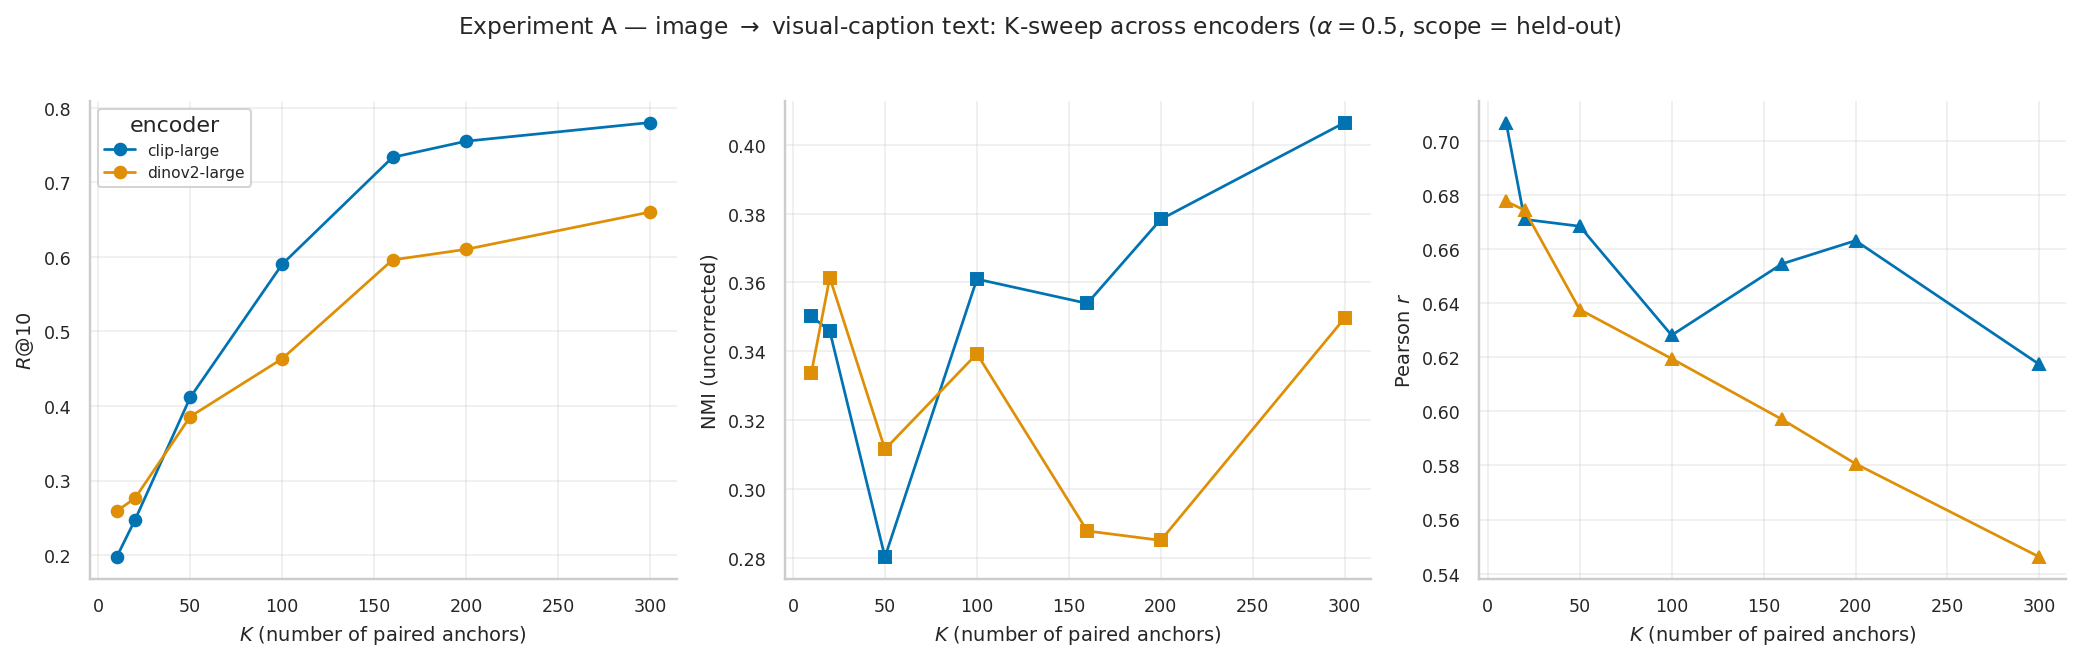
\includegraphics[width=\linewidth]{results/comparison_plots/a__K_sweep_by_encoder.png}
\caption{Experiment~A: cross-encoder $K$-sweep overlay at $\alpha=0.5$, held-out scope. Each curve corresponds to one image encoder, with retrieval and structural metrics shown side by side.}
\label{fig:a-K-sweep-encoders}
\end{figure}

The text-contrastive CLIP encoders outperform the text-free image
encoders at this operating point. CLIP-base slightly outperforms
CLIP-large on held-out retrieval, which may reflect better
regularisation in this small-sample setting rather than a general
advantage of the smaller model. ViT-MAE-base is a useful negative
control: its weak held-out performance suggests that the ridge-FGW
image--caption leg benefits substantially from image--text pretraining.


\section{Within-modality scaffolding: audio $\to$ audio-caption text}
\label{sec:res-b}

Experiment~B fits the same ridge-FGW recipe on
$(\mathcal{Y},\mathcal{Z}^{(Y)})$, with $Y=$ CLAP audio embeddings and
$\mathcal{Z}^{(Y)}=Z^{\text{aud}}$ the per-clip mean of MiniLM-encoded
audio captions. This is the audio-side analogue of Experiment~A and
provides the reusable plan $T_{Y\!Z}$ for the transitive composition.

\subsection{Single-pair view: K\,$\times$\,$\alpha$ sweep}


\begin{table}[!ht]
\centering
\footnotesize
\setlength{\tabcolsep}{3pt}
\resizebox{\textwidth}{!}{%
\begin{tabular}{l ccc ccc ccc ccc ccc}
\toprule
       & \multicolumn{3}{c}{$\alpha = 0.0$} & \multicolumn{3}{c}{$\alpha = 0.3$} & \multicolumn{3}{c}{$\alpha = 0.5$} & \multicolumn{3}{c}{$\alpha = 0.7$} & \multicolumn{3}{c}{$\alpha = 0.9$} \\
        \cmidrule(lr){2-4} \cmidrule(lr){5-7} \cmidrule(lr){8-10} \cmidrule(lr){11-13} \cmidrule(lr){14-16}
$K$ & $R@10$ & NMI & $r$ & $R@10$ & NMI & $r$ & $R@10$ & NMI & $r$ & $R@10$ & NMI & $r$ & $R@10$ & NMI & $r$ \\
\midrule
10 & 0.125 & 0.415 & 0.525 & 0.133 & 0.436 & 0.636 & 0.142 & 0.449 & 0.688 & 0.152 & 0.466 & 0.720 & 0.155 & 0.470 & 0.748 \\
20 & 0.190 & 0.414 & 0.561 & 0.182 & 0.443 & 0.641 & 0.193 & 0.462 & 0.676 & 0.180 & 0.475 & 0.717 & 0.168 & 0.467 & 0.745 \\
50 & 0.278 & 0.416 & 0.554 & 0.275 & 0.415 & 0.615 & 0.273 & 0.419 & 0.651 & 0.260 & 0.446 & 0.696 & 0.212 & 0.455 & 0.737 \\
100 & 0.427 & 0.419 & 0.561 & 0.430 & 0.437 & 0.617 & 0.410 & 0.433 & 0.657 & 0.372 & 0.445 & 0.695 & 0.275 & 0.451 & 0.742 \\
160 & 0.507 & 0.436 & 0.553 & 0.500 & 0.442 & 0.581 & 0.477 & 0.443 & 0.620 & 0.425 & 0.450 & 0.662 & 0.307 & 0.471 & 0.732 \\
200 & 0.573 & 0.425 & 0.543 & 0.568 & 0.439 & 0.574 & 0.535 & 0.428 & 0.609 & 0.482 & 0.450 & 0.659 & 0.350 & 0.483 & 0.733 \\
300 & 0.665 & 0.436 & 0.549 & 0.660 & 0.441 & 0.580 & 0.635 & 0.446 & 0.596 & 0.562 & 0.466 & 0.638 & 0.395 & 0.464 & 0.725 \\
400 & 0.782 & 0.451 & 0.544 & 0.760 & 0.447 & 0.563 & 0.713 & 0.449 & 0.593 & 0.637 & 0.469 & 0.635 & 0.440 & 0.490 & 0.718 \\
\bottomrule
\end{tabular}
}
\caption{Experiment~B --- audio $\to$ audio-caption text: $K\times\alpha$ grid at \textbf{aggregate} scope, evaluated at $(\text{CLAP-HTSAT-unfused}, \text{MiniLM-L6-v2})$. Each cell reports $R@10$ / NMI / Pearson $r$; $K_{\mathrm{cl}}=20$.}
\label{tab:b-grid-agg}
\end{table}

\begin{table}[!ht]
\centering
\footnotesize
\setlength{\tabcolsep}{3pt}
\resizebox{\textwidth}{!}{%
\begin{tabular}{l ccc ccc ccc ccc ccc}
\toprule
       & \multicolumn{3}{c}{$\alpha = 0.0$} & \multicolumn{3}{c}{$\alpha = 0.3$} & \multicolumn{3}{c}{$\alpha = 0.5$} & \multicolumn{3}{c}{$\alpha = 0.7$} & \multicolumn{3}{c}{$\alpha = 0.9$} \\
        \cmidrule(lr){2-4} \cmidrule(lr){5-7} \cmidrule(lr){8-10} \cmidrule(lr){11-13} \cmidrule(lr){14-16}
$K$ & $R@10$ & NMI & $r$ & $R@10$ & NMI & $r$ & $R@10$ & NMI & $r$ & $R@10$ & NMI & $r$ & $R@10$ & NMI & $r$ \\
\midrule
10 & 0.108 & 0.401 & 0.523 & 0.113 & 0.420 & 0.637 & 0.123 & 0.445 & 0.687 & 0.141 & 0.452 & 0.718 & 0.146 & 0.471 & 0.745 \\
20 & 0.147 & 0.417 & 0.563 & 0.139 & 0.442 & 0.643 & 0.155 & 0.442 & 0.677 & 0.153 & 0.449 & 0.715 & 0.155 & 0.445 & 0.742 \\
50 & 0.191 & 0.409 & 0.558 & 0.194 & 0.394 & 0.617 & 0.200 & 0.399 & 0.651 & 0.206 & 0.426 & 0.687 & 0.200 & 0.430 & 0.725 \\
100 & 0.307 & 0.437 & 0.560 & 0.313 & 0.430 & 0.620 & 0.300 & 0.450 & 0.657 & 0.277 & 0.455 & 0.687 & 0.233 & 0.439 & 0.721 \\
160 & 0.304 & 0.442 & 0.570 & 0.317 & 0.450 & 0.602 & 0.304 & 0.422 & 0.633 & 0.283 & 0.434 & 0.656 & 0.237 & 0.445 & 0.694 \\
200 & 0.340 & 0.455 & 0.538 & 0.345 & 0.471 & 0.567 & 0.335 & 0.470 & 0.589 & 0.305 & 0.471 & 0.633 & 0.260 & 0.483 & 0.676 \\
300 & 0.360 & 0.567 & 0.533 & 0.360 & 0.563 & 0.558 & 0.340 & 0.562 & 0.570 & 0.310 & 0.553 & 0.597 & 0.250 & 0.566 & 0.636 \\
400 & \textemdash & \textemdash & \textemdash & \textemdash & \textemdash & \textemdash & \textemdash & \textemdash & \textemdash & \textemdash & \textemdash & \textemdash & \textemdash & \textemdash & \textemdash \\
\bottomrule
\end{tabular}
}
\caption{Experiment~B --- audio $\to$ audio-caption text: $K\times\alpha$ grid at \textbf{held-out} scope, evaluated at $(\text{CLAP-HTSAT-unfused}, \text{MiniLM-L6-v2})$. Each cell reports $R@10$ / NMI / Pearson $r$; $K_{\mathrm{cl}}=20$. The $K=400$ row has no held-out partition by construction.}
\label{tab:b-grid-hel}
\end{table}

\begin{figure}[ht]
\centering
\includegraphics[width=0.95\linewidth]{results/exp_b/sweep.png}
\caption{Experiment~B at the canonical reference pair (CLAP-HTSAT-unfused $\times$ MiniLM): retrieval and structural metrics versus $K$ at $\alpha=0.5$. The aggregate--held-out gap is wider than in Experiment~A, indicating stronger memorisation relative to held-out generalisation on the audio side.}
\label{fig:b-sweep}
\end{figure}

\begin{figure}[ht]
\centering

\includegraphics[width=0.95\linewidth]{results/exp_b/alpha_sweep.png}
\caption{Experiment~B: $\alpha$-sweep at $K=300$ on the canonical reference pair. The retrieval ceiling is lower than in Experiment~A at the same operating point, while Pearson $r$ continues to increase with $\alpha$. This pattern is consistent with the audio-caption leg being harder at the exemplar level while still benefiting structurally from the FGW term.}
\label{fig:b-alpha-sweep}
\end{figure}

\subsection{Cross-pair view: encoder ranking at $K=300$, $\alpha=0.5$}


\begin{table}[!ht]
\centering
\small
\setlength{\tabcolsep}{5pt}
\begin{tabular}{r l l c c c}
\toprule
Rank & Image encoder & Audio encoder & $R@10$ & NMI & Pearson $r$ \\
\midrule
\textbf{1} & \textbf{---} & \textbf{clap-larger} & \textbf{0.470} & \textbf{0.572} & \textbf{0.604} \\
2 & --- & clap-fused & 0.350 & 0.537 & 0.526 \\
3 & --- & clap-unfused & 0.340 & 0.562 & 0.570 \\
4 & --- & mert-95m & 0.200 & 0.511 & 0.512 \\
5 & --- & mert-330m & 0.080 & 0.508 & 0.496 \\
\bottomrule
\end{tabular}
\caption{Experiment~B: top 5 audio encoders by held-out $R@10$ at $K=300$, $\alpha=0.5$. The image column is not applicable because this is an audio--text experiment.}
\label{tab:b-encoders}
\end{table}

\begin{figure}[ht]
\centering
\includegraphics[width=0.48\linewidth]{results/exp_grid/plots/b_R10_by_audio_encoder.png}
\hfill
\includegraphics[width=0.48\linewidth]{results/exp_grid/plots/b_NMI_by_audio_encoder.png}
\caption{Experiment~B across audio encoders. Left: $R@10$ at $K=300$, $\alpha=0.5$, aggregate versus held-out. Right: NMI. CLAP encoders dominate retrieval, while the MERT family retains competitive cluster-level structure but weak exemplar identity.}
\label{fig:b-encoder-bars}
\end{figure}

\begin{figure}[ht]
\centering
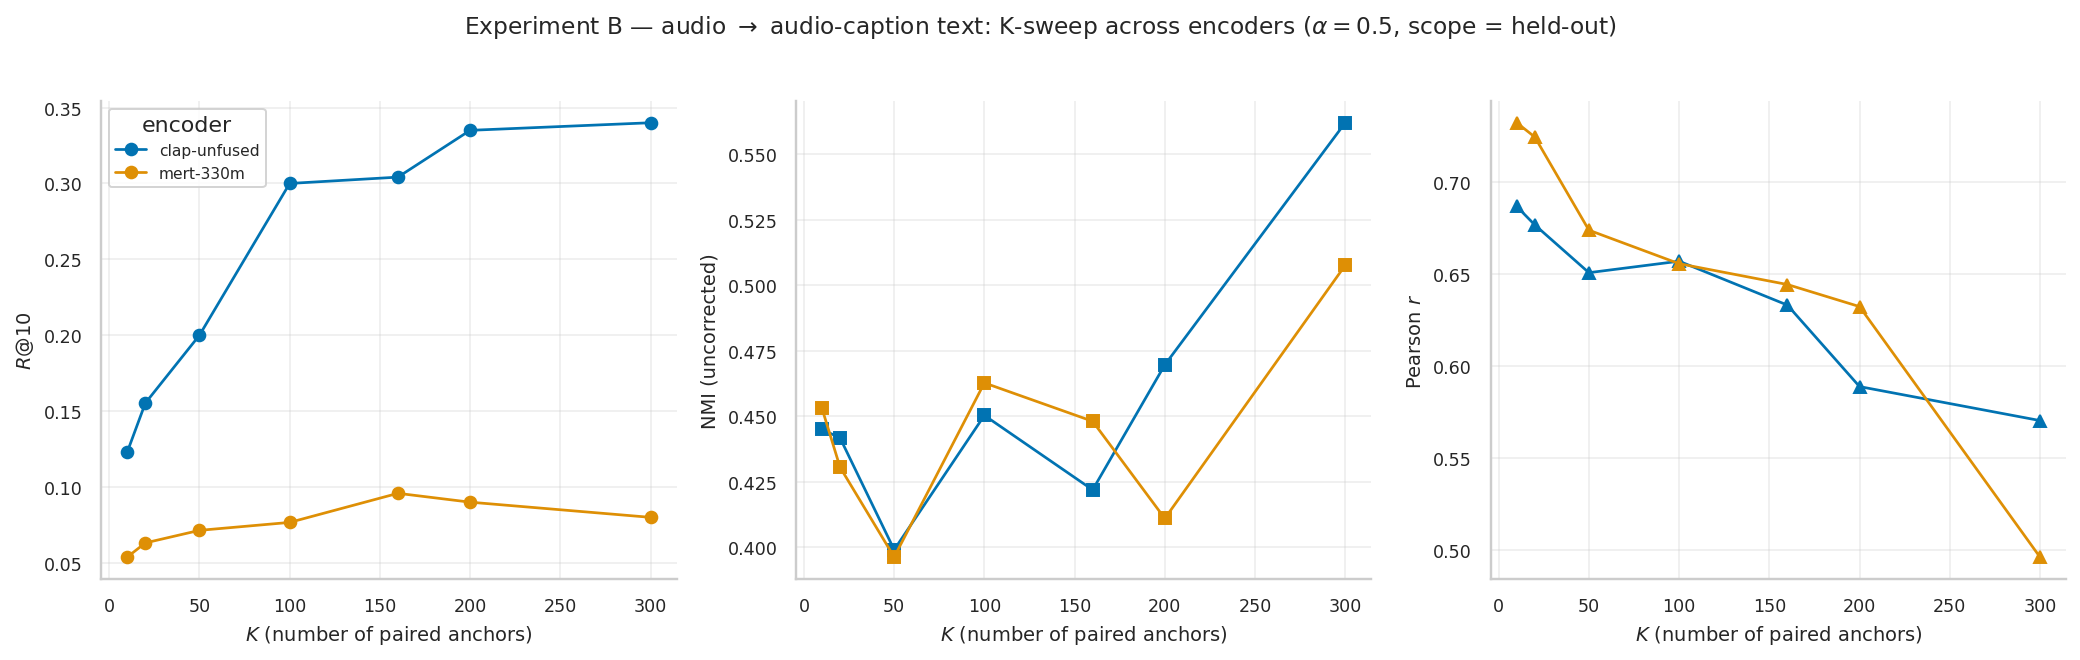
\includegraphics[width=\linewidth]{results/comparison_plots/b__K_sweep_by_encoder.png}
\caption{Experiment~B: cross-encoder $K$-sweep overlay at $\alpha=0.5$, held-out scope. Each curve corresponds to one audio encoder.}
\label{fig:b-K-sweep-encoders}
\end{figure}

The largest CLAP variant gives the best retrieval. The MERT encoders
are weaker for exemplar-level audio--caption retrieval, but their NMI
and Pearson scores remain non-trivial. This suggests that MERT retains
useful audio-domain geometry even when it is not arranged to recover
caption identity through the ridge-FGW leg.


\section{Supervised linear reference: C-direct}
\label{sec:res-cdirect}

C-direct fits a closed-form ridge map from $X$ to $Y$ on $K=300$ real
$\mathcal{X}\leftrightarrow\mathcal{Y}$ anchors and combines it with
the intra-modal costs $C_1,C_2$ through FGW. It is the only directly
paired image--audio recipe in the chapter. It should be interpreted as
a \emph{supervised linear reference}, not as a universal supervised
ceiling: its performance reflects the capacity and regularisation of a
linear ridge map in this low-data setting.

\subsection{Single-pair view: K-sweep at the canonical pair}


\begin{table}[!ht]
\centering
\footnotesize
\setlength{\tabcolsep}{3pt}
\resizebox{\textwidth}{!}{%
\begin{tabular}{l ccc ccc ccc ccc ccc}
\toprule
       & \multicolumn{3}{c}{$\alpha = 0.0$} & \multicolumn{3}{c}{$\alpha = 0.3$} & \multicolumn{3}{c}{$\alpha = 0.5$} & \multicolumn{3}{c}{$\alpha = 0.7$} & \multicolumn{3}{c}{$\alpha = 0.9$} \\
        \cmidrule(lr){2-4} \cmidrule(lr){5-7} \cmidrule(lr){8-10} \cmidrule(lr){11-13} \cmidrule(lr){14-16}
$K$ & $R@10$ & NMI & $r$ & $R@10$ & NMI & $r$ & $R@10$ & NMI & $r$ & $R@10$ & NMI & $r$ & $R@10$ & NMI & $r$ \\
\midrule
10 & 0.082 & 0.277 & 0.159 & 0.085 & 0.276 & 0.377 & 0.069 & 0.284 & 0.476 & 0.069 & 0.272 & 0.555 & 0.051 & 0.312 & 0.643 \\
20 & 0.095 & 0.286 & 0.231 & 0.087 & 0.280 & 0.413 & 0.087 & 0.281 & 0.516 & 0.089 & 0.313 & 0.587 & 0.047 & 0.308 & 0.638 \\
50 & 0.123 & 0.286 & 0.265 & 0.137 & 0.292 & 0.373 & 0.131 & 0.274 & 0.491 & 0.126 & 0.281 & 0.532 & 0.089 & 0.287 & 0.599 \\
100 & 0.183 & 0.245 & 0.256 & 0.173 & 0.261 & 0.352 & 0.173 & 0.253 & 0.425 & 0.147 & 0.269 & 0.531 & 0.100 & 0.285 & 0.597 \\
160 & 0.250 & 0.315 & 0.330 & 0.254 & 0.318 & 0.433 & 0.246 & 0.303 & 0.451 & 0.237 & 0.290 & 0.523 & 0.121 & 0.297 & 0.598 \\
200 & 0.225 & 0.287 & 0.289 & 0.250 & 0.282 & 0.389 & 0.245 & 0.285 & 0.441 & 0.230 & 0.296 & 0.494 & 0.145 & 0.308 & 0.597 \\
300 & 0.320 & 0.408 & 0.272 & 0.320 & 0.390 & 0.295 & 0.320 & 0.396 & 0.346 & 0.250 & 0.429 & 0.459 & 0.110 & 0.416 & 0.553 \\
400 & \textemdash & \textemdash & \textemdash & \textemdash & \textemdash & \textemdash & \textemdash & \textemdash & \textemdash & \textemdash & \textemdash & \textemdash & \textemdash & \textemdash & \textemdash \\
\bottomrule
\end{tabular}
}
\caption{Experiment~C-direct --- image $\to$ audio, supervised linear reference: $K\times\alpha$ grid at \textbf{held-out} scope, evaluated at $(\text{CLIP-L/14}, \text{CLAP-HTSAT-unfused})$. Each cell reports $R@10$ / NMI / Pearson $r$; $K_{\mathrm{cl}}=15$. The $K=400$ row has no held-out partition by construction.}
\label{tab:cdirect-K-hel}
\end{table}

\subsection{Reference-pair comparison}


\begin{table}[!ht]
\centering
\small
\setlength{\tabcolsep}{5pt}
\begin{tabular}{l l ccc ccc}
\toprule
Encoder pair & Role & \multicolumn{3}{c}{Aggregate} & \multicolumn{3}{c}{Held-out} \\
        \cmidrule(lr){3-5} \cmidrule(lr){6-8}
 &  & $R@10$ & NMI & $r$ & $R@10$ & NMI & $r$ \\
\midrule
CLIP-L/14 $\times$ CLAP-unfused & text-aligned & 0.790 & 0.248 & 0.306 & 0.320 & 0.396 & 0.346 \\
DINOv2-large $\times$ MERT-330m & text-free & 0.608 & 0.290 & 0.467 & 0.060 & 0.451 & 0.524 \\
\bottomrule
\end{tabular}
\caption{Experiment~C-direct at the two reference encoder pairs, $K=300$, $\alpha=0.5$. Each cell reports $R@10$ / NMI / Pearson $r$. The held-out $R@10$ values should be compared to the held-out candidate-pool chance rate rather than the full 400-row chance rate.}
\label{tab:cdirect-refpairs}
\end{table}

On the text-aligned pair, C-direct reaches held-out $R@10=0.320$. On
the text-free pair it drops to $R@10=0.060$, which is below the
$0.10$ chance rate if the held-out candidate pool contains 100 rows.
In either interpretation, the drop is large. The result supports a
limited conclusion: in this low-data linear-ridge setting, direct
image--audio supervision generalises much better when the encoders
already expose a compatible text-aligned geometry. It does not imply
that all supervised image--audio alignment would fail on text-free
encoders.

\subsection{Cross-pair view: encoder ranking}


\begin{table}[!ht]
\centering
\small
\setlength{\tabcolsep}{5pt}
\begin{tabular}{r l l c c c}
\toprule
Rank & Image encoder & Audio encoder & $R@10$ & NMI & Pearson $r$ \\
\midrule
\textbf{1} & \textbf{clip-large} & \textbf{clap-larger} & \textbf{0.390} & \textbf{0.399} & \textbf{0.334} \\
2 & clip-large & clap-unfused & 0.320 & 0.396 & 0.346 \\
3 & clip-base & clap-larger & 0.310 & 0.435 & 0.300 \\
4 & clip-large & clap-fused & 0.290 & 0.390 & 0.398 \\
5 & clip-base & clap-fused & 0.280 & 0.428 & 0.275 \\
6 & dinov2-large & clap-larger & 0.280 & 0.392 & 0.331 \\
7 & dinov2-large & clap-unfused & 0.250 & 0.403 & 0.431 \\
8 & dinov2-large & clap-fused & 0.220 & 0.371 & 0.399 \\
\bottomrule
\end{tabular}
\caption{Experiment~C-direct: top 8 encoder pairs by held-out $R@10$. Each row is evaluated at the recipe's canonical operating point. The best cells use CLIP and CLAP encoders, consistent with the supervised linear reference benefiting from inherited text-aligned structure.}
\label{tab:cdirect-encoders}
\end{table}

\begin{figure}[ht]
\centering
\includegraphics[width=0.95\linewidth]{results/exp_c/sweep.png}
\caption{C-direct at the canonical reference pair: $K$-sweep showing the widening aggregate--held-out gap. The held-out curve plateaus near $0.32$ from $K=160$ onward, while aggregate performance continues to rise. This is evidence of memorisation under the ridge map, not a general supervised ceiling.}
\label{fig:cdirect-sweep}
\end{figure}

\begin{figure}[ht]
\centering
\includegraphics[width=0.48\linewidth]{results/exp_grid/plots/cdirect_R10_heldout.png}
\hfill
\includegraphics[width=0.48\linewidth]{results/exp_grid/plots/cdirect_R10_aggregate.png}
\caption{C-direct $R@10$ heatmaps across the $6\times5$ encoder grid. Left: held-out scope. Right: aggregate scope. Rows are image encoders, columns are audio encoders. The strongest held-out cells use text-aligned encoders; text-free DINOv2$\times$MERT pairs are weak under this linear supervised reference.}
\label{fig:cdirect-heatmaps}
\end{figure}

\begin{figure}[ht]
\centering
\includegraphics[width=0.7\linewidth]{results/exp_grid/plots/delta_c_minus_d_R10.png}
\caption{Difference between C-direct and D in $R@10$, $R^{\text{C-direct}}_{10}-R^{\text{D}}_{10}$, at each encoder pair. Positive cells indicate settings where the directly supervised linear reference beats caption-cost FGW; negative cells indicate settings where the weak-bridge recipe is stronger. The pattern suggests that direct ridge supervision is most useful on text-aligned encoder pairs, while D is more robust elsewhere.}
\label{fig:cdirect-delta}
\end{figure}


\section{Weak-bridge caption-cost FGW: Experiment~D}
\label{sec:res-d}

Experiment~D realises the weak-bridge construction of
\S\ref{sec:weak-bridge}. The cross-modal cost $M$ is built from visual
and audio caption embeddings, while the intra-modal costs $C_1,C_2$
come from the image and audio embeddings. The recipe uses no direct
$\mathcal{X}\leftrightarrow\mathcal{Y}$ anchors. It should therefore
be described as \emph{text-mediated} or \emph{weak-bridge} alignment,
not as fully unsupervised alignment. The only strictly no-caption,
no-label, geometry-only condition in this chapter is Pure-GW.

\subsection{Single-pair view: $\alpha$ ablation at the canonical pair}


\begin{table}[!ht]
\centering
\footnotesize
\setlength{\tabcolsep}{3pt}
\resizebox{\textwidth}{!}{%
\begin{tabular}{l ccc ccc ccc ccc ccc}
\toprule
       & \multicolumn{3}{c}{$\alpha = 0.0$} & \multicolumn{3}{c}{$\alpha = 0.3$} & \multicolumn{3}{c}{$\alpha = 0.5$} & \multicolumn{3}{c}{$\alpha = 0.7$} & \multicolumn{3}{c}{$\alpha = 0.9$} \\
        \cmidrule(lr){2-4} \cmidrule(lr){5-7} \cmidrule(lr){8-10} \cmidrule(lr){11-13} \cmidrule(lr){14-16}
$K$ & $R@10$ & NMI & $r$ & $R@10$ & NMI & $r$ & $R@10$ & NMI & $r$ & $R@10$ & NMI & $r$ & $R@10$ & NMI & $r$ \\
\midrule
0 & 0.205 & 0.262 & 0.258 & 0.220 & 0.190 & 0.198 & 0.228 & 0.202 & 0.310 & 0.225 & 0.224 & 0.427 & 0.203 & 0.270 & 0.552 \\
\bottomrule
\end{tabular}
}
\caption{Experiment~D --- weak-bridge caption-cost FGW: $K\times\alpha$ grid at \textbf{aggregate} scope, evaluated at $(\text{CLIP-L/14}, \text{CLAP-HTSAT-unfused})$. Each cell reports $R@10$ / NMI / Pearson $r$; $K_{\mathrm{cl}}=15$. $K=0$ because D uses no direct image--audio anchors; only $\alpha$ varies.}
\label{tab:d-alpha-agg}
\end{table}

\subsection{Reference-pair comparison}


\begin{table}[!ht]
\centering
\small
\setlength{\tabcolsep}{5pt}
\begin{tabular}{l l ccc ccc}
\toprule
Encoder pair & Role & \multicolumn{3}{c}{Aggregate} & \multicolumn{3}{c}{Same-rows} \\
        \cmidrule(lr){3-5} \cmidrule(lr){6-8}
 &  & $R@10$ & NMI & $r$ & $R@10$ & NMI & $r$ \\
\midrule
CLIP-L/14 $\times$ CLAP-unfused & text-aligned & 0.225 & 0.224 & 0.427 & 0.267 & 0.736 & 0.374 \\
DINOv2-large $\times$ MERT-330m & text-free & 0.223 & 0.200 & 0.356 & 0.192 & 0.762 & 0.440 \\
\bottomrule
\end{tabular}
\caption{Experiment~D at the two reference encoder pairs, $\alpha=0.7$. Each cell reports $R@10$ / NMI / Pearson $r$. Same-rows retrieval should be compared to the same-rows candidate-pool chance rate; for a 100-row pool this is $0.10$.}
\label{tab:d-refpairs}
\end{table}

On the text-free reference pair, D reaches same-rows $R@10=0.192$.
If the same-rows candidate pool contains 100 items, this is about
$1.9\times$ chance rather than $8\times$ chance. The stronger evidence
for D is therefore not a large identity-retrieval margin, but the
combination of above-chance retrieval with high NMI and higher Pearson
$r$ than the Text-only baseline on the same reference pair. This
supports the interpretation that the caption bridge supplies the
cross-modal matching signal, while the FGW structural term regularises
or reshapes the plan toward better category and distance consistency.

\subsection{Cross-pair view: encoder ranking}


\begin{table}[!ht]
\centering
\small
\setlength{\tabcolsep}{5pt}
\begin{tabular}{r l l c c c}
\toprule
Rank & Image encoder & Audio encoder & $R@10$ & NMI & Pearson $r$ \\
\midrule
\textbf{1} & \textbf{clip-base} & \textbf{mert-95m} & \textbf{0.423} & \textbf{0.696} & \textbf{0.407} \\
2 & clip-large & mert-330m & 0.391 & 0.779 & 0.410 \\
3 & clip-base & mert-330m & 0.350 & 0.734 & 0.096 \\
4 & clip-large & clap-fused & 0.348 & 0.767 & 0.375 \\
5 & vit-mae-base & clap-larger & 0.346 & 0.706 & 0.104 \\
6 & clip-large & mert-95m & 0.323 & 0.685 & 0.600 \\
7 & dinov2-base & mert-95m & 0.318 & 0.793 & 0.252 \\
8 & clip-base & clap-fused & 0.304 & 0.745 & 0.177 \\
\bottomrule
\end{tabular}
\caption{Experiment~D: top 8 encoder pairs by same-rows $R@10$. Each row is evaluated at the recipe's canonical operating point. Because the same-rows partition contains few samples, differences of a few hundredths in $R@10$ should be interpreted cautiously unless supported by bootstrap or paired tests.}
\label{tab:d-encoders}
\end{table}

\begin{figure}[ht]
\centering
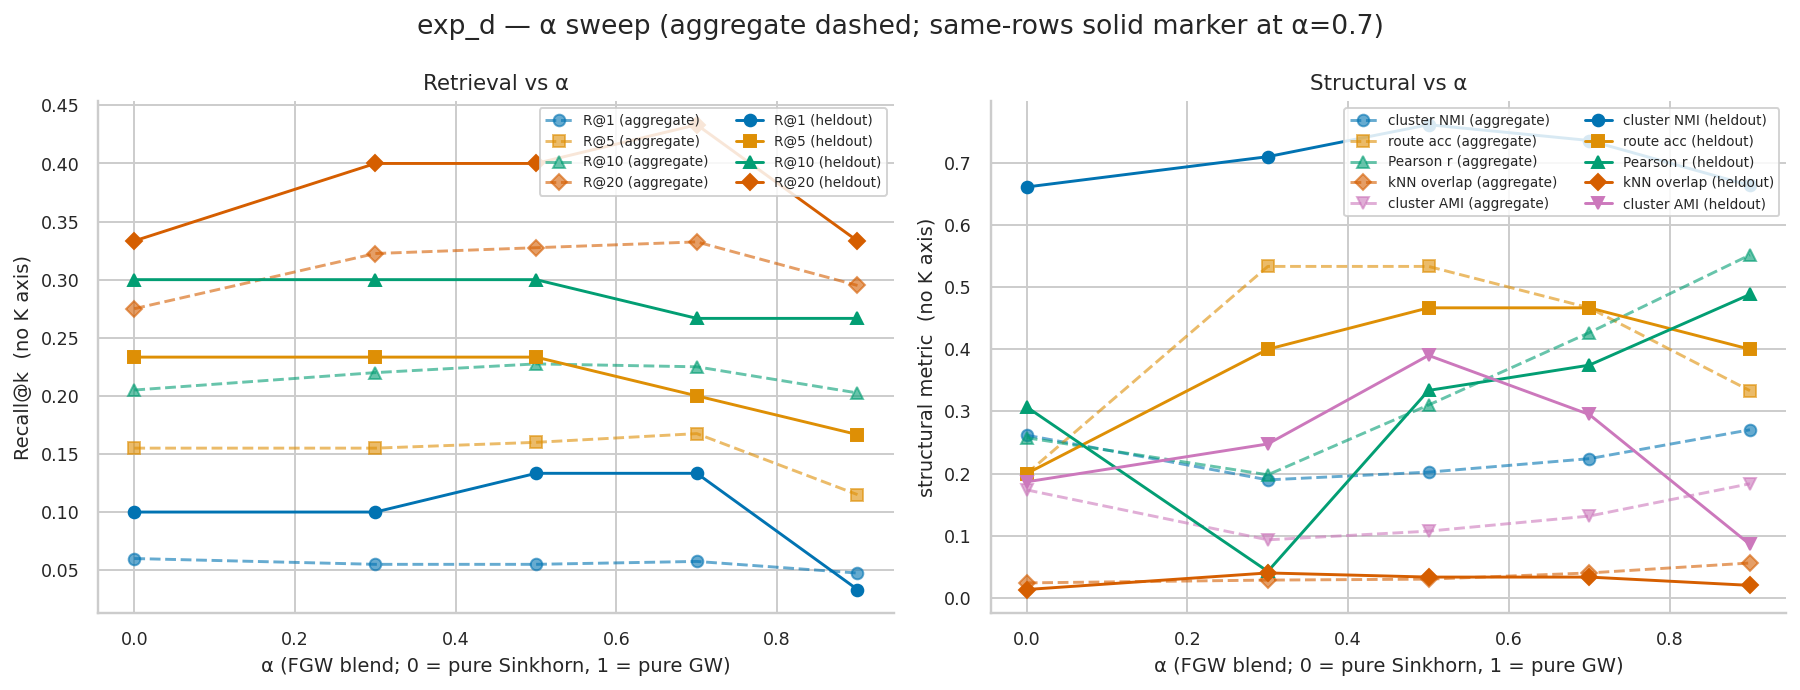
\includegraphics[width=0.95\linewidth]{results/exp_d/alpha_sweep.png}
\caption{D at the canonical reference pair: $\alpha$ ablation. Aggregate $R@10$ is relatively flat across $\alpha$, while Pearson $r$ rises with the structural weight. The available metrics therefore suggest that the FGW structural term contributes more to distance consistency than to exact row identity.}
\label{fig:d-alpha-sweep}
\end{figure}

\begin{figure}[ht]
\centering
\includegraphics[width=0.48\linewidth]{results/exp_grid/plots/d_R10_sameRows.png}
\hfill
\includegraphics[width=0.48\linewidth]{results/exp_grid/plots/d_NMI_sameRows.png}
\caption{Experiment~D heatmaps across the encoder grid, same-rows scope. Left: $R@10$. Right: NMI. Strong cells include MERT audio encoders, which suggests that D can benefit from self-supervised intra-modal audio geometry when the cross-modal signal is supplied by captions.}
\label{fig:d-heatmaps}
\end{figure}

\begin{figure}[ht]
\centering
\includegraphics[width=0.7\linewidth]{results/exp_grid/plots/delta_d_minus_text_R10.png}
\caption{Difference between D and the Text-only baseline, $R^{\text{D}}_{10}-R^{\text{Text}}_{10}$, at each encoder pair. Positive cells indicate settings where FGW improves retrieval over raw caption cosine; cells near zero indicate that the transport solve mainly changes structural consistency rather than identity retrieval.}
\label{fig:d-delta}
\end{figure}

D's best audio encoder is MERT-95m, which is weak in the supervised
audio--caption leg of Experiment~B. This is not a contradiction. In D,
the captions provide the inter-modal cost $M$, while the audio encoder
contributes the intra-modal geometry $C_2$. A self-supervised audio
encoder can therefore be weak at caption identity retrieval yet useful
as a structural cost for FGW. The result supports an intra/inter
separation: the best encoder for cross-modal feature matching need not
be the best encoder for within-modality geometry.


\section{Pure entropic Gromov--Wasserstein}
\label{sec:res-gw}

Pure-GW omits the cross-modal cost $M$ entirely and aligns the two
intra-modal distance matrices under entropic GW. This is the only
strictly geometry-only condition in the chapter: no labels, no
captions, and no direct image--audio anchors are supplied to the
transport solve.

\subsection{Reference-pair comparison}


\begin{table}[!ht]
\centering
\small
\setlength{\tabcolsep}{5pt}
\begin{tabular}{l l ccc ccc}
\toprule
Encoder pair & Role & \multicolumn{3}{c}{Aggregate} & \multicolumn{3}{c}{Same-rows} \\
        \cmidrule(lr){3-5} \cmidrule(lr){6-8}
 &  & $R@10$ & NMI & $r$ & $R@10$ & NMI & $r$ \\
\midrule
CLIP-L/14 $\times$ CLAP-unfused & text-aligned & 0.020 & 0.374 & 0.672 & 0.067 & 0.715 & 0.564 \\
DINOv2-large $\times$ MERT-330m & text-free & 0.060 & 0.401 & 0.655 & 0.038 & 0.727 & 0.656 \\
\bottomrule
\end{tabular}
\caption{Pure entropic GW at the two reference encoder pairs, equivalent to $\alpha=1$ with no cross-modal feature cost. Each cell reports $R@10$ / NMI / Pearson $r$. High NMI and Pearson values should be interpreted as proxy evidence for structural compatibility; the full GW-specific distortion metrics are not yet reported in this table.}
\label{tab:gw-refpairs}
\end{table}

Pure-GW produces the clearest structure--identity separation. Retrieval
is near or below the 100-row chance rate when evaluated on same-rows,
whereas NMI and Pearson $r$ are high relative to the other
cross-modal recipes. This is consistent with the invariances of GW:
without a cross-modal feature cost, the solver can preserve relational
or cluster-level structure without recovering the true exemplar
pairing. The result should therefore be stated as category/geometry
alignment, not identity alignment.

\subsection{Cross-pair view: encoder ranking}


\begin{table}[!ht]
\centering
\small
\setlength{\tabcolsep}{5pt}
\begin{tabular}{r l l c c c}
\toprule
Rank & Image encoder & Audio encoder & $R@10$ & NMI & Pearson $r$ \\
\midrule
\textbf{1} & \textbf{dinov2-base} & \textbf{clap-larger} & \textbf{0.172} & \textbf{0.593} & \textbf{0.030} \\
2 & dinov2-base & clap-unfused & 0.161 & 0.672 & 0.180 \\
3 & dinov2-base & clap-fused & 0.143 & 0.528 & 0.086 \\
4 & dinov2-base & mert-95m & 0.136 & 0.656 & 0.390 \\
5 & clip-large & clap-larger & 0.097 & 0.730 & 0.488 \\
6 & clip-large & clap-fused & 0.087 & 0.757 & 0.353 \\
7 & clip-base & clap-unfused & 0.087 & 0.744 & 0.404 \\
8 & dinov2-small & mert-330m & 0.083 & 0.782 & 0.695 \\
\bottomrule
\end{tabular}
\caption{Pure-GW: top 8 encoder pairs by same-rows $R@10$. Retrieval remains weak even for the best cells; the main evidence for Pure-GW is structural rather than identity-level.}
\label{tab:gw-encoders}
\end{table}

\begin{figure}[ht]
\centering
\includegraphics[width=0.48\linewidth]{results/exp_grid/plots/unsup_R10_aggregate.png}
\hfill
\includegraphics[width=0.48\linewidth]{results/exp_grid/plots/unsup_NMI_sameRows.png}
\caption{Pure-GW heatmaps. Left: aggregate $R@10$. Right: same-rows NMI. The NMI heatmap is high for several self-supervised image encoders, but because NMI is uncorrected and has a non-negligible chance floor, this plot should be read as evidence of coarse cluster compatibility rather than exact semantic recovery.}
\label{fig:gw-heatmaps}
\end{figure}

DINOv2-base is the dominant image encoder by same-rows retrieval in
this grid, although the absolute retrieval values remain low. The
more robust conclusion is that self-supervised image geometry appears
useful to Pure-GW's structural objective. On the audio side, CLAP
variants perform well in the ranking, but the differences are small
relative to the sample size.


\section{Text-only retrieval baseline}
\label{sec:res-text}

The Text-only baseline bypasses optimal transport and ranks target rows
by the raw cosine similarity of the visual-caption and audio-caption
embeddings. This is an important baseline because Experiment~D also
uses captions to define its cross-modal cost. Therefore, D's retrieval
scores should always be compared against Text-only before attributing
improvements to the FGW solve.

\subsection{Reference-pair comparison}


\begin{table}[!ht]
\centering
\small
\setlength{\tabcolsep}{5pt}
\begin{tabular}{l l ccc ccc}
\toprule
Encoder pair & Role & \multicolumn{3}{c}{Aggregate} & \multicolumn{3}{c}{Same-rows} \\
        \cmidrule(lr){3-5} \cmidrule(lr){6-8}
 &  & $R@10$ & NMI & $r$ & $R@10$ & NMI & $r$ \\
\midrule
CLIP-L/14 $\times$ CLAP-unfused & text-aligned & 0.233 & 0.258 & 0.315 & 0.300 & 0.683 & 0.347 \\
DINOv2-large $\times$ MERT-330m & text-free & 0.233 & 0.193 & 0.247 & 0.192 & 0.627 & 0.282 \\
\bottomrule
\end{tabular}
\caption{Text-only baseline at the two reference encoder pairs. The retrieval plan is defined by caption cosine rather than by image or audio encoders; the structural metrics differ because they are computed using the image and audio embedding geometries.}
\label{tab:text-refpairs}
\end{table}

At the two reference pairs, Text-only is a strong retrieval baseline.
On CLIP$\times$CLAP, it reaches same-rows $R@10=0.300$, higher than D's
$0.267$. On DINOv2$\times$MERT, it matches D at $R@10=0.192$. D's
advantage at the reference pairs is therefore not identity retrieval;
it is the higher structural agreement on the text-free pair, especially
NMI and Pearson $r$. This supports the interpretation that the FGW
solve changes the geometry of the plan, but it does not by itself show
a consistent retrieval improvement over caption cosine.

\subsection{Cross-pair view: encoder ranking}


\begin{table}[!ht]
\centering
\small
\setlength{\tabcolsep}{5pt}
\begin{tabular}{r l l c c c}
\toprule
Rank & Image encoder & Audio encoder & $R@10$ & NMI & Pearson $r$ \\
\midrule
\textbf{1} & \textbf{clip-large} & \textbf{mert-95m} & \textbf{0.387} & \textbf{0.637} & \textbf{0.135} \\
2 & vit-mae-base & clap-unfused & 0.321 & 0.746 & 0.014 \\
3 & dinov2-small & mert-95m & 0.308 & 0.703 & 0.128 \\
4 & vit-mae-base & clap-larger & 0.308 & 0.697 & 0.104 \\
5 & clip-base & mert-95m & 0.308 & 0.730 & 0.274 \\
6 & clip-large & mert-330m & 0.304 & 0.695 & -0.077 \\
7 & clip-large & clap-unfused & 0.300 & 0.683 & 0.347 \\
8 & clip-large & clap-larger & 0.290 & 0.741 & 0.383 \\
\bottomrule
\end{tabular}
\caption{Text-only baseline: top 8 encoder pairs by same-rows $R@10$. Since the caption-cosine retrieval plan is encoder-independent, variation in this table should be read as arising from the same-rows evaluation subset, candidate filtering, or implementation details of the grid evaluation. If the same rows are intended to be identical across encoder pairs, this table should be regenerated before making encoder-ranking claims from Text-only retrieval.}
\label{tab:text-encoders}
\end{table}

\begin{figure}[ht]
\centering
\includegraphics[width=0.7\linewidth]{results/exp_grid/plots/text_R10_aggregate.png}
\caption{Text-only aggregate $R@10$ heatmap. Because the caption-cosine plan is encoder-independent, aggregate retrieval should be constant across the encoder grid when the evaluated rows and candidate pool are identical.}
\label{fig:text-heatmap}
\end{figure}

The Text-only baseline is therefore not a minor control; it is a strong
competitor for retrieval. The added value of D should be framed in
terms of structural consistency and robustness across encoders, with
retrieval gains claimed only in cells where the improvement over
Text-only is larger than the expected sampling noise.


\section{Transitive composition through text}
\label{sec:res-ctrans}

C-transitive composes the within-modality reusable plans $T_{X\!Z}$
from Experiment~A and $T_{Y\!Z}$ from Experiment~B through a text
bridge in $\mathcal{Z}$. Because the composition requires fitting both
within-modality legs on the same encoder swap, the encoder grid is not
reported for C-transitive; the table below gives the canonical
reference pair.


\begin{table}[!ht]
\centering
\small
\setlength{\tabcolsep}{5pt}
\begin{tabular}{l c c c c}
\toprule
Scope & $R@10$ & NMI & AMI & Pearson $r$ \\
\midrule
Aggregate & 0.175 & 0.302 & 0.220 & 0.484 \\
Held-out  & 0.067 & 0.776 & 0.465 & 0.555 \\
\bottomrule
\end{tabular}
\caption{C-transitive at the canonical reference pair (CLIP-L/14 $\times$ CLAP-HTSAT-unfused), per-leg $K_{\text{leg}}=300$, $\alpha_{\text{leg}}=0.7$; bridge top-$k=20$, softmax temperature $\tau=0.1$. AMI is reported where available from the per-experiment sweep CSV.}
\label{tab:c-trans-canonical}
\end{table}

C-transitive is the strongest example of structure without identity in
the current results. Held-out $R@10=0.067$ is weak under a 100-row
chance rate of $0.10$, but NMI and AMI are high. This indicates that
the composed text bridge preserves category-level structure while
averaging over many caption neighbours and losing exemplar identity.
The availability of AMI here makes this claim stronger than the
uncorrected-NMI claims elsewhere in the chapter.


\section{Cross-method synthesis}
\label{sec:res-synthesis}


\begin{table}[!ht]
\centering
\small
\setlength{\tabcolsep}{5pt}
\begin{tabular}{l cc cc cl}
\toprule
      & \multicolumn{2}{c}{CLIP $\times$ CLAP}      & \multicolumn{2}{c}{DINOv2 $\times$ MERT}      & \multicolumn{2}{c}{Configuration optimum} \\
        \cmidrule(lr){2-3} \cmidrule(lr){4-5} \cmidrule(lr){6-7}
Method & $R@10$ & NMI & $R@10$ & NMI & $R@10$ & Best pair \\
\midrule
C-direct (supervised linear, $K=300$) & 0.320 & 0.396 & 0.060 & 0.451 & 0.390 & clip-large $\times$ clap-larger \\
D (caption-cost FGW) & 0.267 & 0.736 & 0.192 & 0.762 & 0.423 & clip-base $\times$ mert-95m \\
Pure-GW & 0.067 & 0.715 & 0.038 & 0.727 & 0.172 & dinov2-base $\times$ clap-larger \\
Text-only (cosine) & 0.300 & 0.683 & 0.192 & 0.627 & 0.387 & clip-large $\times$ mert-95m \\
\bottomrule
\end{tabular}
\caption{Cross-method summary at the two reference encoder pairs and at each recipe's configuration optimum. $R@10$ and NMI are reported on the held-out / same-rows partition. If this partition contains 100 candidates, the chance baseline for $R@10$ is $0.10$. NMI is uncorrected and should be interpreted relative to the approximate chance floor of $0.36$ for $n=100$, $K_{\mathrm{cl}}=15$.}
\label{tab:cross-method-summary}
\end{table}

\begin{figure}[ht]
\centering
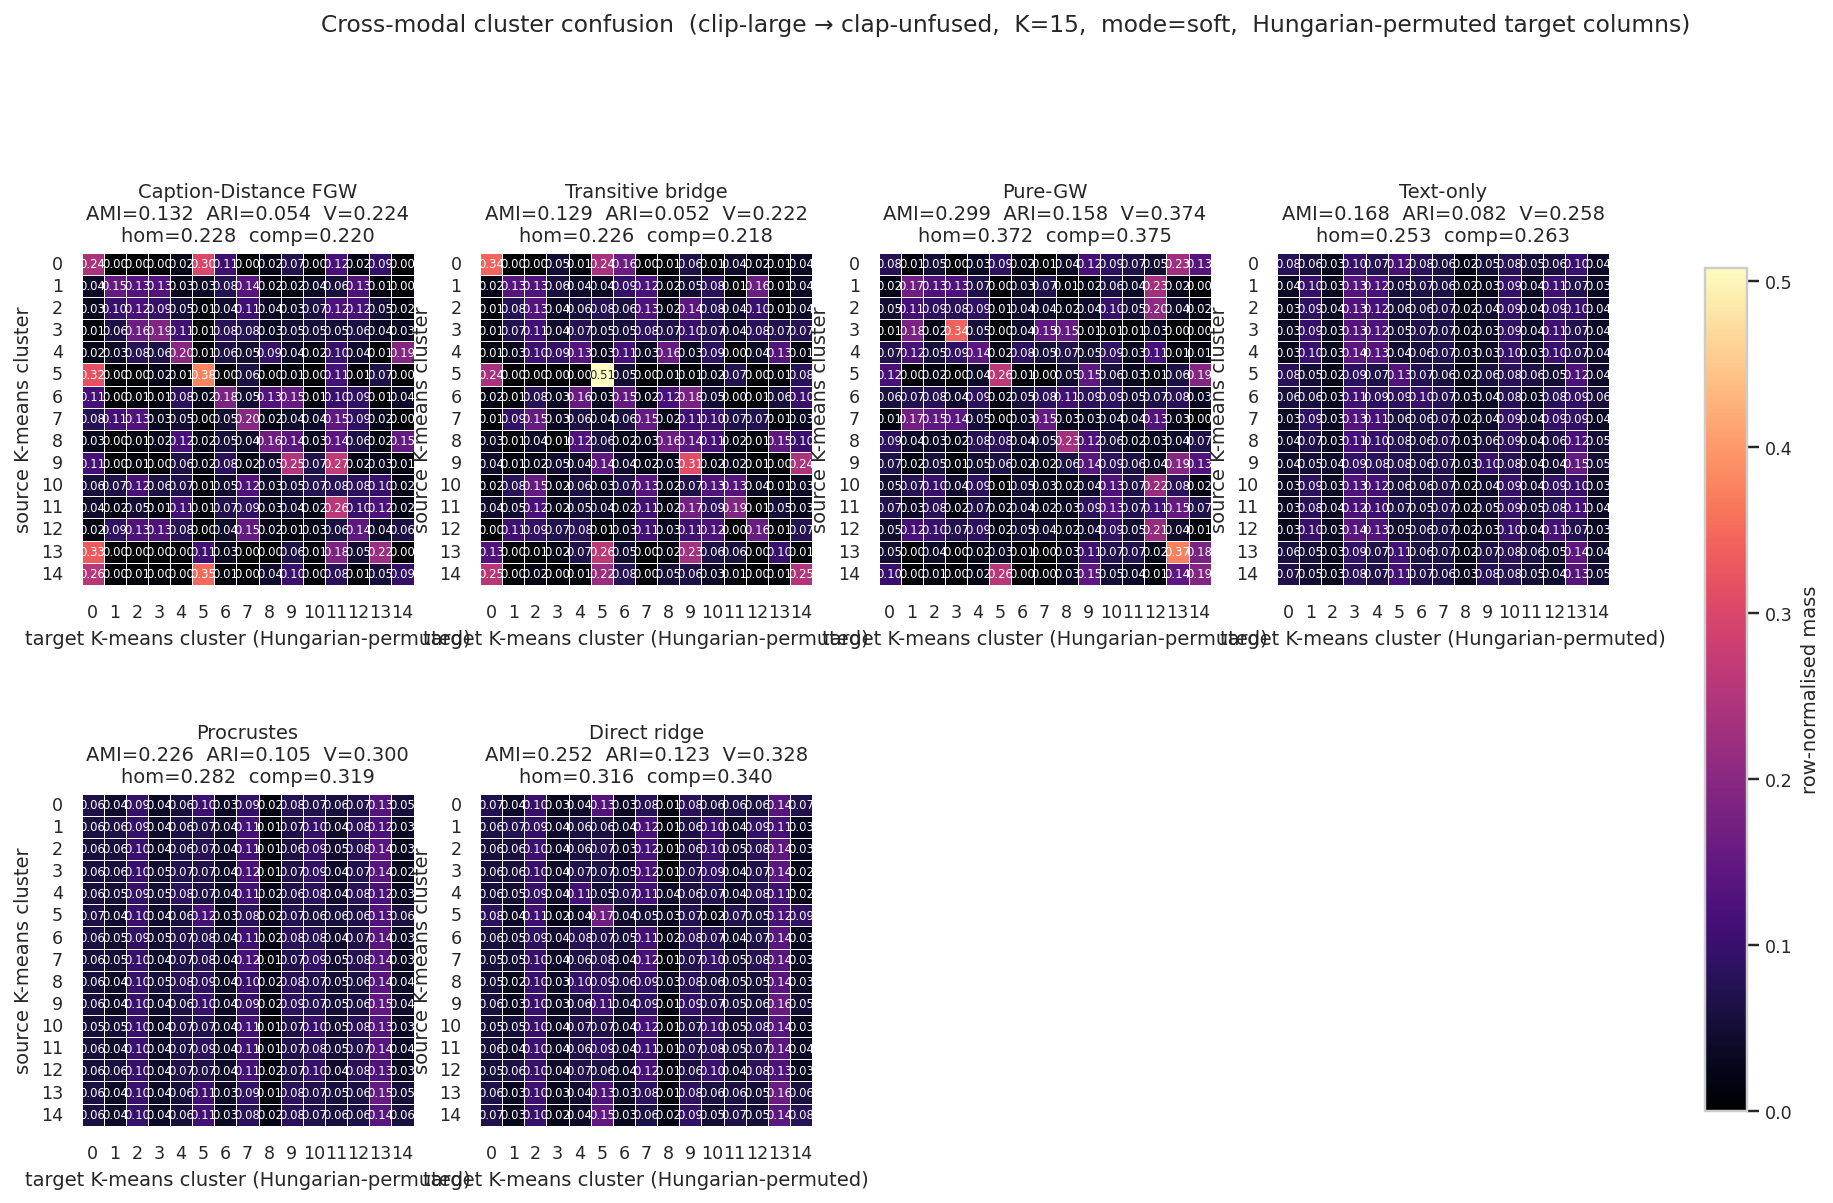
\includegraphics[width=\linewidth]{results/exp_grid/plots/cross_modal_cluster_confusions__K15_soft.png}
\caption{Cross-modal cluster confusion matrices for the four cross-modal recipes at the canonical reference pair, $K_{\mathrm{cl}}=15$, Hungarian-permuted so the diagonal is dominant. A block-diagonal matrix indicates cleaner categorical alignment; a smeared matrix indicates cluster fragmentation. The subplot annotations report chance-corrected cluster-agreement scalars where available, making this figure more reliable than uncorrected NMI alone.}
\label{fig:cluster-confusion}
\end{figure}

\begin{figure}[ht]
\centering
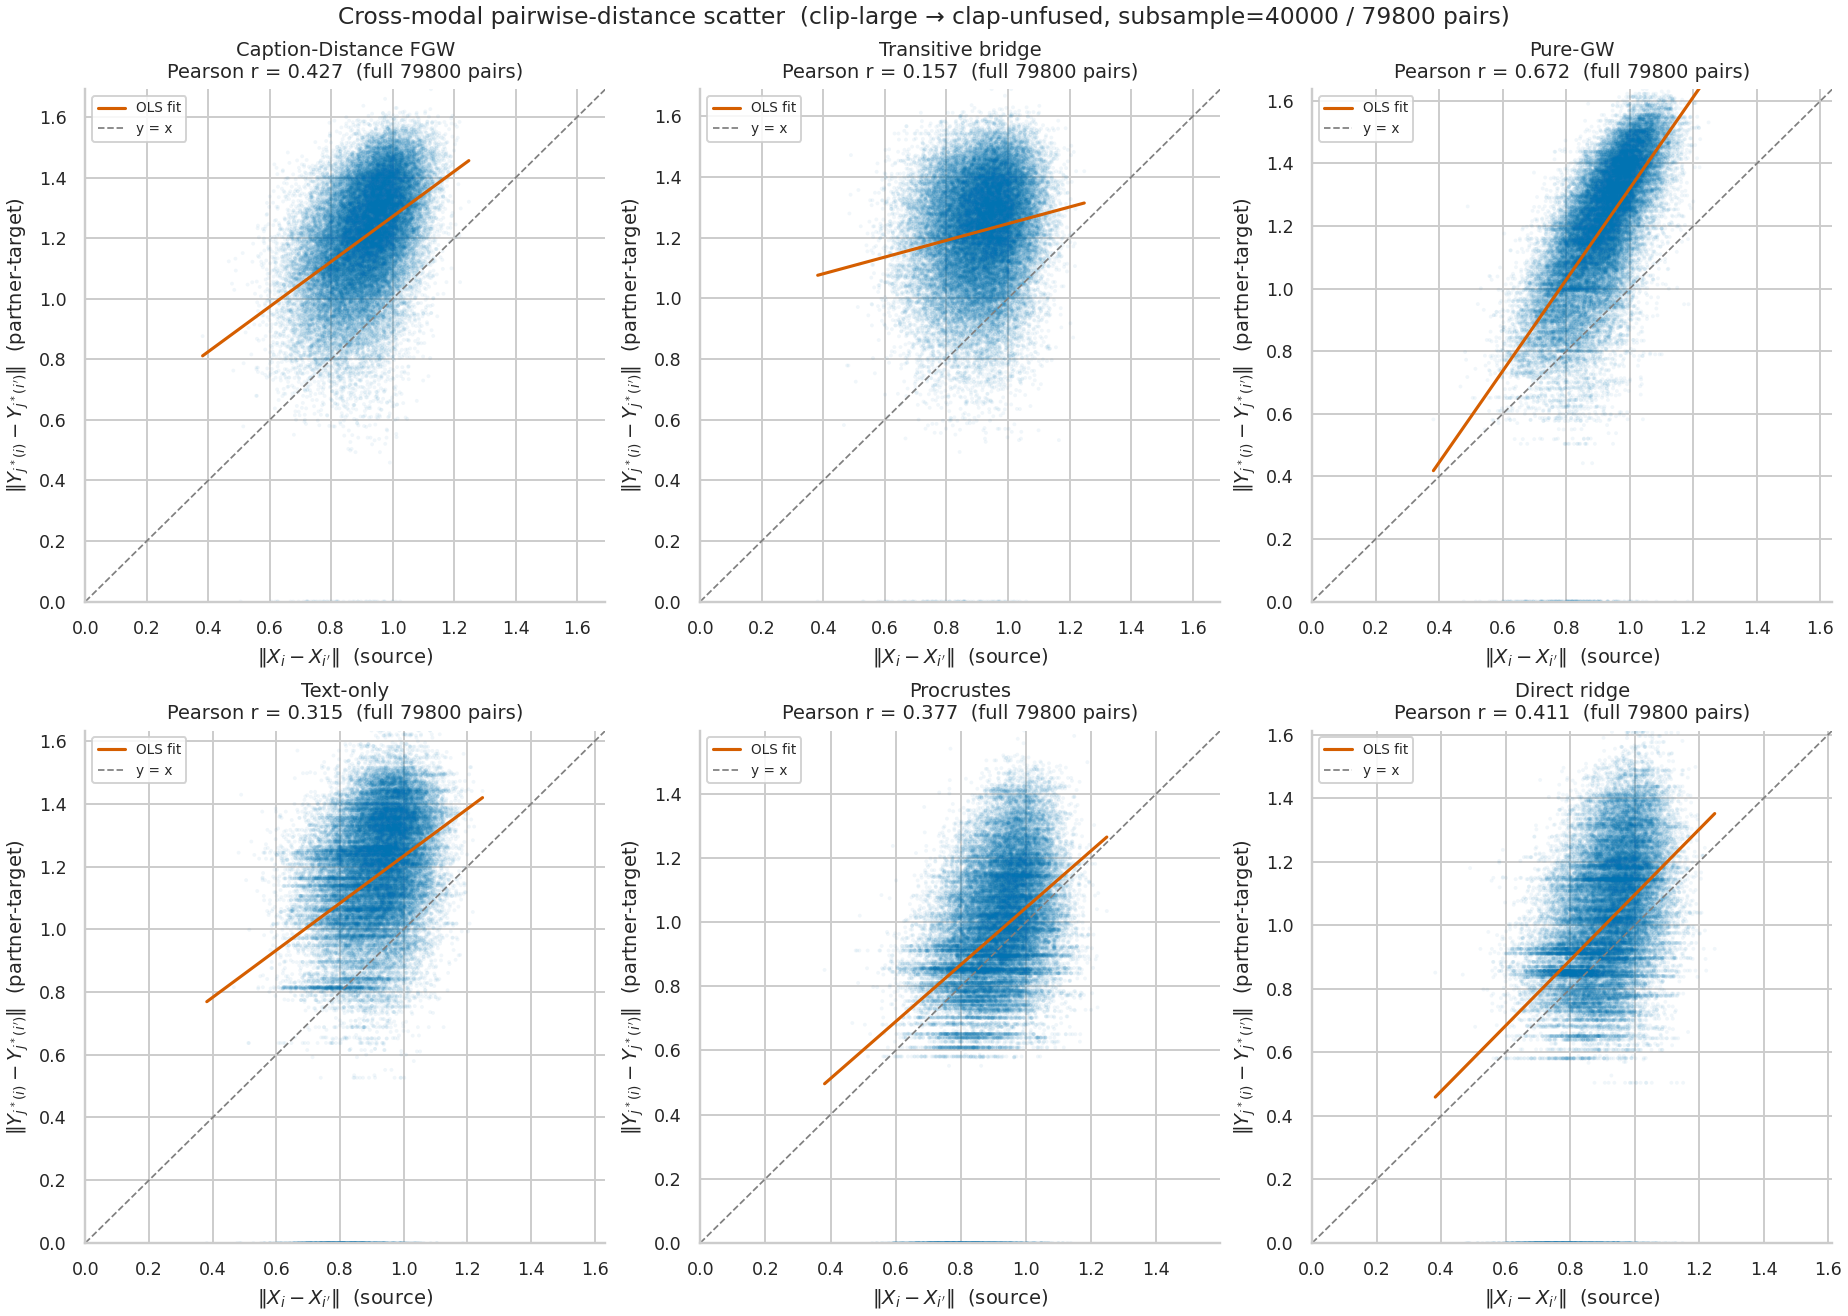
\includegraphics[width=\linewidth]{results/exp_grid/plots/cross_modal_pearson_scatter.png}
\caption{Cross-modal pairwise-distance scatter for the four cross-modal recipes at the canonical reference pair. For each plan $T$, the partner mapping $\hat\jmath(i)=\arg\max_j T_{ij}$ is decoded, and source-space pairwise distances $\|X_i-X_{i'}\|$ are plotted against target-space partner distances $\|Y_{\hat\jmath(i)}-Y_{\hat\jmath(i')}\|$. A tighter positive band indicates stronger distance preservation under the decoded map. This is a useful proxy for geometric preservation, but it should eventually be complemented by normalized GW distortion and coupling diagnostics.}
\label{fig:pearson-scatter}
\end{figure}

Table~\ref{tab:cross-method-summary} shows a consistent separation
between identity retrieval and structural agreement. C-direct is the
strongest directly supervised linear reference on the text-aligned pair
but drops sharply on the text-free pair. D maintains non-trivial
same-rows retrieval on the text-free pair and improves structural
agreement relative to Text-only, but it does not consistently beat
Text-only in retrieval at the two reference pairs. Pure-GW has weak
retrieval but high NMI and Pearson $r$, supporting the interpretation
that geometry-only GW recovers coarse relational structure rather than
exemplar identity.

The configuration-optimum column should be interpreted cautiously. On a
100-row evaluation, the difference between D's optimum $R@10=0.423$ and
C-direct's optimum $R@10=0.390$ corresponds to only a few additional
queries. This ranking is suggestive, but a paired test or bootstrap
confidence interval is needed before treating the gap as statistically
meaningful.

\paragraph{Main empirical takeaway.}
The experiments support a structure--identity decoupling. Direct linear
supervision recovers exemplar identity mainly when the encoders are
already compatible, while geometry-driven methods preserve category or
distance structure more reliably than identity. Caption-cost FGW sits
between these extremes: it uses captions as a weak cross-modal bridge
and FGW as a structural regulariser, giving stronger category/geometry
agreement than Text-only in several settings but not a uniformly better
retrieval score.


\section{Summary of empirical findings}
\label{sec:res-summary}

\begin{itemize}
  \item \textbf{C-direct is highly encoder-dependent in this low-data
  linear setting.} On CLIP$\times$CLAP it reaches held-out
  $R@10=0.320$, but on DINOv2$\times$MERT it drops to $R@10=0.060$.
  This supports the claim that the linear supervised reference relies
  heavily on compatible encoder geometry; it should not be read as a
  universal limitation of supervised cross-modal alignment.

  \item \textbf{D is best described as weak-bridge, text-mediated FGW.}
  It uses no direct image--audio anchors, but it does use captions to
  build the cross-modal cost. On the text-free reference pair it reaches
  same-rows $R@10=0.192$, which is above a 100-row chance rate of
  $0.10$, and it improves structural agreement over Text-only. Its
  clearest contribution is therefore geometric/category consistency,
  not a uniform retrieval gain over caption cosine.

  \item \textbf{Pure-GW recovers structure without identity.} Its
  retrieval scores are near chance, but NMI and Pearson $r$ are high.
  This is the expected behaviour of a geometry-only GW method: without
  an external cross-modal anchor, the coupling can preserve relational
  structure while failing to identify the true paired exemplar.

  \item \textbf{Text-only is a strong baseline.} At the two reference
  pairs, Text-only matches or exceeds D on $R@10$. Any claim that FGW
  improves retrieval should therefore be made relative to this baseline
  and supported by uncertainty estimates. D's stronger claim is that it
  can improve structural consistency over the caption-only plan.

  \item \textbf{Different recipes prefer different encoder pairs.}
  C-direct prefers text-aligned CLIP/CLAP configurations; D can prefer
  MERT on the audio side because captions supply the cross-modal cost
  and the audio encoder mainly supplies $C_2$; Pure-GW favours encoders
  with useful intra-modal geometry. This supports the proposed
  separation between inter-modal anchoring and intra-modal structure.
\end{itemize}

The next revision should add GW-native diagnostics---normalized GW
loss, feature cost, structural cost, entropy, marginal violation,
hubness, local neighborhood preservation, and cycle consistency---so
that the geometric claims can be tested directly rather than through
NMI and Pearson proxies alone.
